\input{preamble.tex}
\newcommand{\C}{\mathcal{C}}

\begin{document}
\pagestyle{fancy}
\fancyhead[L]{Seconde}
\fancyhead[C]{\textbf{DS n°3 — fonctions numériques}}
\fancyhead[R]{\today}

\reversemarginpar

\null\vspace{-30pt}
Nom / Prénom : \\

Consignes particulières : 
\begin{itemize}[label=$\bullet$]
	\item 
	La calculatrice est {interdite}.
	\item 
	L'exercice \ref{exe:1} peut être fait entièrement sur la feuille d'évaluation. Écrire son nom avant de rendre le sujet pour qu'il soit corrigé.
	\item 
	Toute trace de recherche est prise en compte.
	\item 
	L'abbréviation $\tq$ signifie ``tel que''.
\end{itemize}

\hrule

\exe{4}{
	Vrai ou faux ? Cocher la case correspondante (aucune justification n'est attendue). \\
	\vspace{-20pt}
	\begin{center}
	\begin{tabular}{c c c}
		\hspace{10cm} & Vrai & Faux \\
		Soit $f$ une fonction numérique. Il existe nécessairement un antécédent de 0 par $f$ & \resizebox{10pt}{!}{$\square$} & \resizebox{10pt}{!}{$\square$}   \\
		$2 \in ]-2;3[$ & \resizebox{10pt}{!}{$\square$} & \resizebox{10pt}{!}{$\square$}   \\
		Un intervalle de $\R$ contient nécessairement un nombre entier (positif ou négatif) & \resizebox{10pt}{!}{$\square$} & \resizebox{10pt}{!}{$\square$}   \\
		On a $\N \subset \Q$ & \resizebox{10pt}{!}{$\square$} & \resizebox{10pt}{!}{$\square$}   \\
	\end{tabular}
	\end{center}
}{exe:1}{
Les réponses sont, dans l'ordre : Faux, vrai, faux, vrai.
}

\exe{5}{
Résoudre dans $\R$ les équations suivantes :
\begin{multicols}{3}
\begin{enumerate}[label=(\alph*)]
\item $5x - 60 = 0$ 
\item $7x + 9 = 3$ 
\item $\frac{x}4 - 2 = \frac13$
\item $x - 3 = \frac27 x + \frac34$
\item $12 \times \left ( \frac{x}3 + \frac14 \right ) = 11$ 
\end{enumerate}
\end{multicols}
}{exe:2}{
\begin{multicols}{3}
\begin{enumerate}[label=(\alph*)]
\item $x=12$ 
\item $x=-\frac67$ 
\item $x=\frac{28}3$
\item $x=\frac{21}4$
\item $x=2$ 
\end{enumerate}
\end{multicols}
}

\exe{4}{
On considère le programme de calcul suivant :
\begin{enumerate}[label=(\roman*)]
\item On prend un nombre réel \textbf{strictement positif}.
\item On mutiplie ce nombre par $\frac73$.
\item On ajoute $-\frac14$ à ce nombre.
\end{enumerate}
Peut-on modéliser ce programme de calcul par une fonction ? Si oui :
\begin{enumerate}
\item Donner son domaine de définition.
\item Donner sa forme algébrique.
\item Donner les éventuels antécédents du point $0$ par la fonction.
\item Représenter une partie de la courbe représentative de la fonction dans un repère.
\end{enumerate}
}{exe:3}{
Le programme peut être modélisé par une fonction que l'on note $f$.
\begin{enumerate}
\item $\D_f = ]0 ; \infty [$.
\item $f(x) = \frac73x -\frac14$.
\item $f(x) = 0 \iff x = \frac{3}{28}$.
\item 
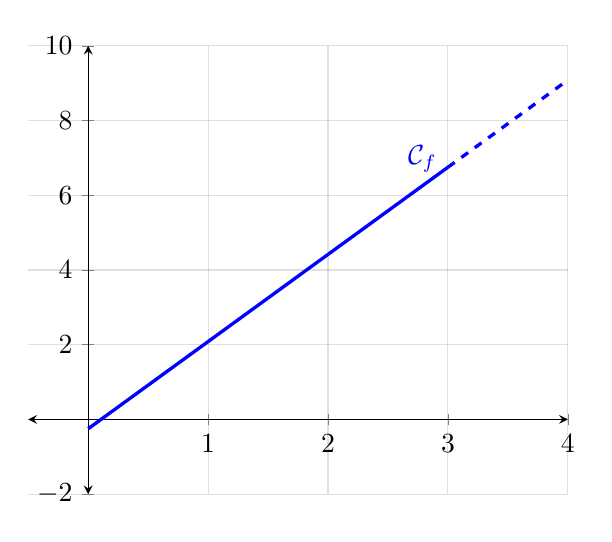
\begin{tikzpicture}[>=stealth, scale=1]
	\begin{axis}[xmin = -0.5, xmax=4, ymin=-2, ymax=10, axis x line=middle, axis y line=middle, axis line style=<->, xlabel={}, ylabel={}, 		grid=both, grid style = {opacity=.5}]]

	\addplot[blue, very thick, domain =-0:3, samples=2] {7*x/3-1/4}  node[above=3pt, left] {$\C_f$};
	\addplot[blue, very thick, dashed, domain =3:4, samples=2] {7*x/3-1/4};

\end{axis}
\end{tikzpicture}
\end{enumerate}
}
	
\exe{4}{
On considère la fonction $g$ définie par :
\[ \begin{array}{c c c c}
g : & \R & \to & \R \\
& x & \mapsto & x^2 + 2
\end{array} \]

\begin{enumerate}
\item Donner l'image de 5 par la fonction $g$.
\item Existe-t-il un réel différent de $5$ dont l'image par $g$ est égale à $g(5)$ ? Si oui, donner ce réel.
\item Donner les éventuels antécédents de 11 par la fonction $g$.
\item Existe-t-il un réel $x$ tel que $g(x) <2$ ? Justifier.
\end{enumerate}
}{exe:4}{
\begin{enumerate}
\item $g(5)=27$.
\item Comme le carré ignore les signes, $g(-5)=27=g(5)$.
\item $g(x)=11 \iff x = 3 \text{ ou } x=-3$.
\item Comme $x^2 \geq 0$, on a nécessairement $g(x) \geq 2$. Donc $g(x) < 2$ est impossible.
\end{enumerate}
}

\newpage

\exe{3}{
On considère les intervalles $I_1 = ] -5 ; 3]$ et $I_2 = [-3 ; 4[$ et $x$ une variable réelle.
\begin{enumerate}
\item Traduire l'appartenance de $x$ aux intervalles $I_1$ et $I_2$ en termes d'inégalités.
\item Donner une condtion pour que $x$ appartienne à l'intervalle $I_1$ \textbf{ET} à l'intervalle $I_2$.
\item Expliciter l'intervalle $I_1 \cap I_2$.
\end{enumerate}
}{exe:5}{
\begin{enumerate}
\item $x \in I_1 \iff -5 < x \leq 3$ ; $x \in I_2 \iff -3 \leq x < 4$.
\item $x \in I_1 \text{ ET } x \in I_2 \iff -3 \leq x \leq 3$.
\item $I_1 \cap I_2 = [-3 ; 3]$.
\end{enumerate}
}

\exe{}{
(Exercice bonus) \\
Déterminer une fonction numérique $g$, définie sur $\R$, et telle que :
\[ g(0) = 1 \quad ; \quad g(-1) = 2 \quad ; \quad g(1) = 2 \]
}{exe:b}{
La fonction définie sur $\R$ par $g(x) = x^2+1$ convient.
}

%%%%%%%%%%%%

\newpage
\fancyhead[C]{\textbf{Solutions}}
\shipoutAnswer

\end{document}
 